\section{Experimental results}

As we have defined earlier, a decoding failure is an instance where, on input $(H,s)$, where $s$ is of the form $s=He^T$, the syndrome decoder output $e'$ is such that $He'^T \ne s$ or $e' \ne e$.  The experiment was also designed to record any decoding instances where $He'^T=s$ and $e'\ne e$, but none were discovered. 

\todo{Updated data available}
\begin{table}[ht]
    \begin{center}
        \begin{tabular}{c|c|c|r}
            \;\;\;$r$\;\;\; & \;Decoding failures\;  & \;Decoding trials\;  & \;$\log_2(\mathrm{DFR})$ \\
            \hline
            389 & 939 & $10^3$ & $-0.09$ \\
            419 & 680 & $10^3$ & $-0.56$ \\
            421 & 652 & $10^3$ & $-0.62$ \\
            443 & 3289 & $10^4$ & $-1.60$ \\
            461 & 1172 & $10^4$ & $-3.09$ \\
            467 & 850 & $10^4$ & $-3.56$ \\
            491 & 1524 & $10^5$ & $-6.04$ \\
            509 & 380 & $10^5$ & $-8.04$ \\
            523 & 946 & $10^6$ & $-10.05$ \\
            541 & 164 & $10^6$ & $-12.57$ \\
            547 & 70 & $10^6$ & $-13.80$ \\
            557 & 177 & $10^7$ & $-15.79$ \\
            563 & 108 & $10^7$ & $-16.50$ \\
            587 & 128 & $10^8$ & $-19.58$ \\
            613 & 61 & $10^8$ & $-20.64$ \\
            619 & 60 & $10^8$ & $-20.67$ \\
            653 & 37 & $10^8$ & $-21.37$ \\
            659 & 35 & $10^8$ & $-21.45$ \\
            661 & 37 & $10^8$ & $-21.37$ \\
            677 & 24 & $10^8$ & $-21.99$ \\
            701 & 20 & $10^8$ & $-22.25$ \\
            757 & 8 & $10^8$ & $-23.58$ \\
            827 & 7 & $10^8$ & $-23.77$
        \end{tabular}
    \end{center}
    \caption{Decoding failure rates for $r$-values such that $389 \leq r \leq 827$, $r$ is prime, and $x^r - 1$ has only two irreducible factors modulo $2$. The data was computed using the parameters and methods described above.}
    \label{table:DFR}
\end{table}

For the security level $\lambda = 20$, we manage to reproduce the error floor region as predicted in \cite{Richardson03}.

\begin{figure}[htbp]
  \begin{center}
    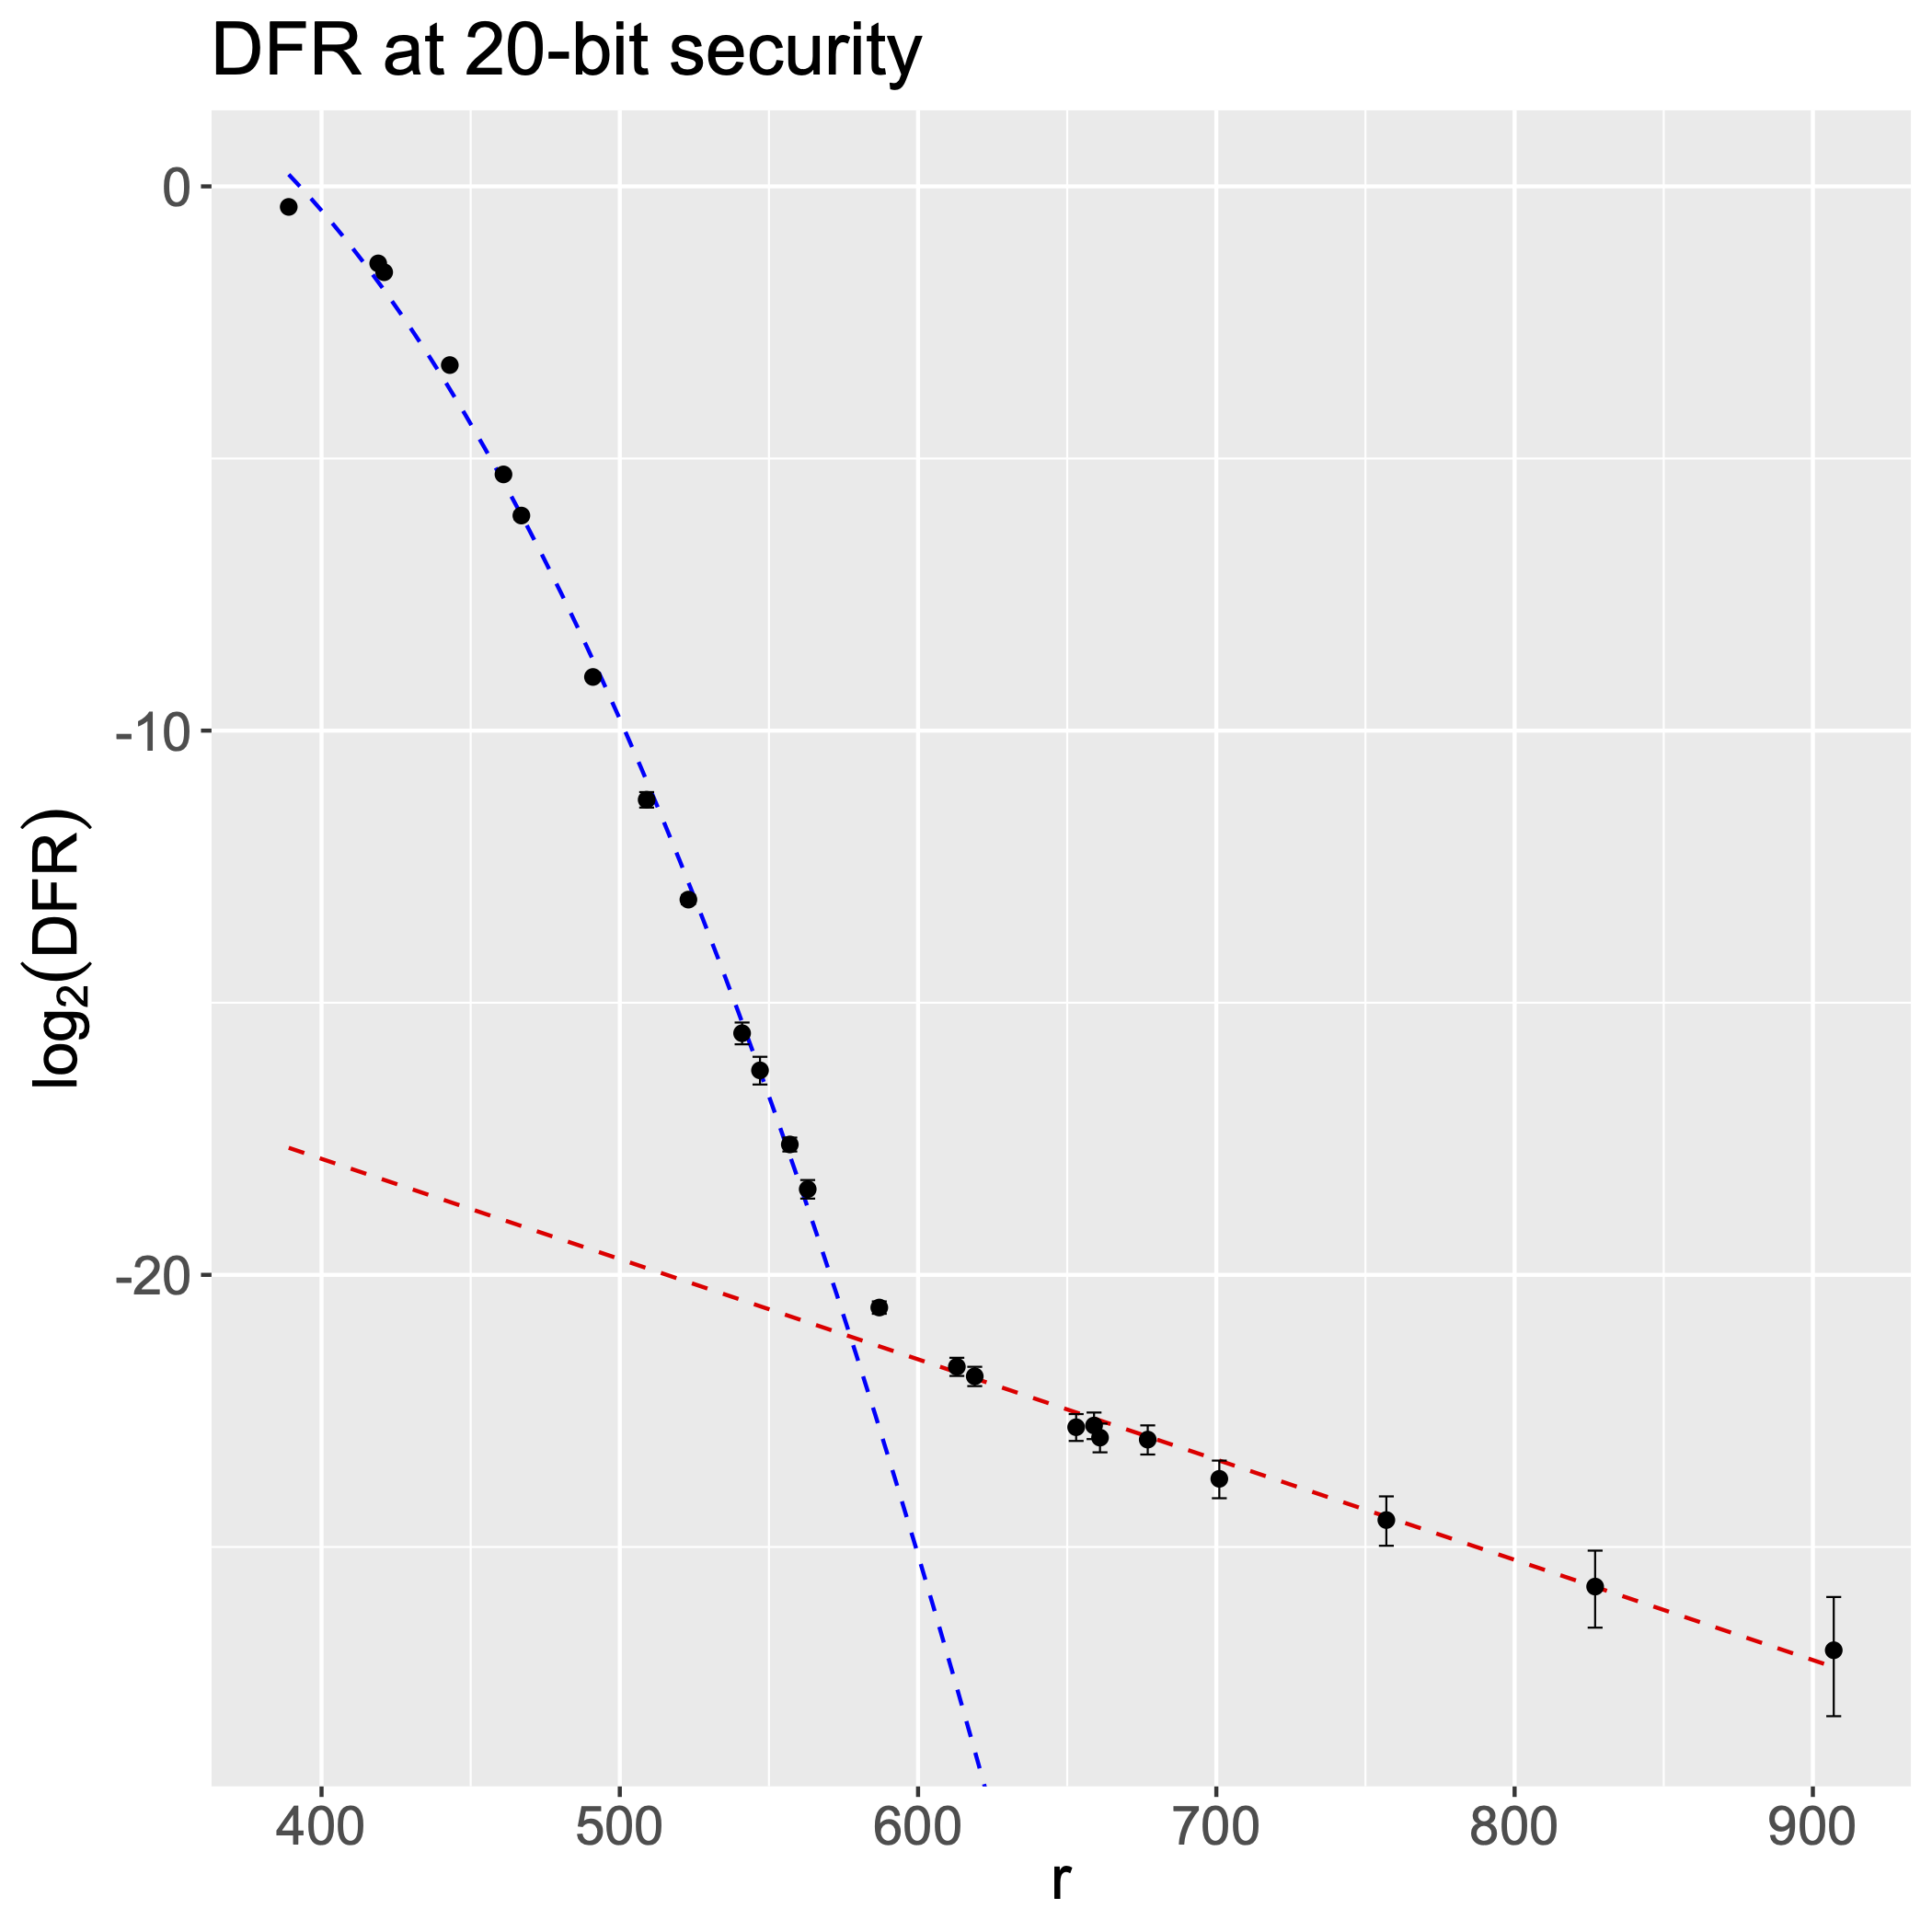
\includegraphics[width=0.49\textwidth]{2_bike/DFR-plot-T3.png}
    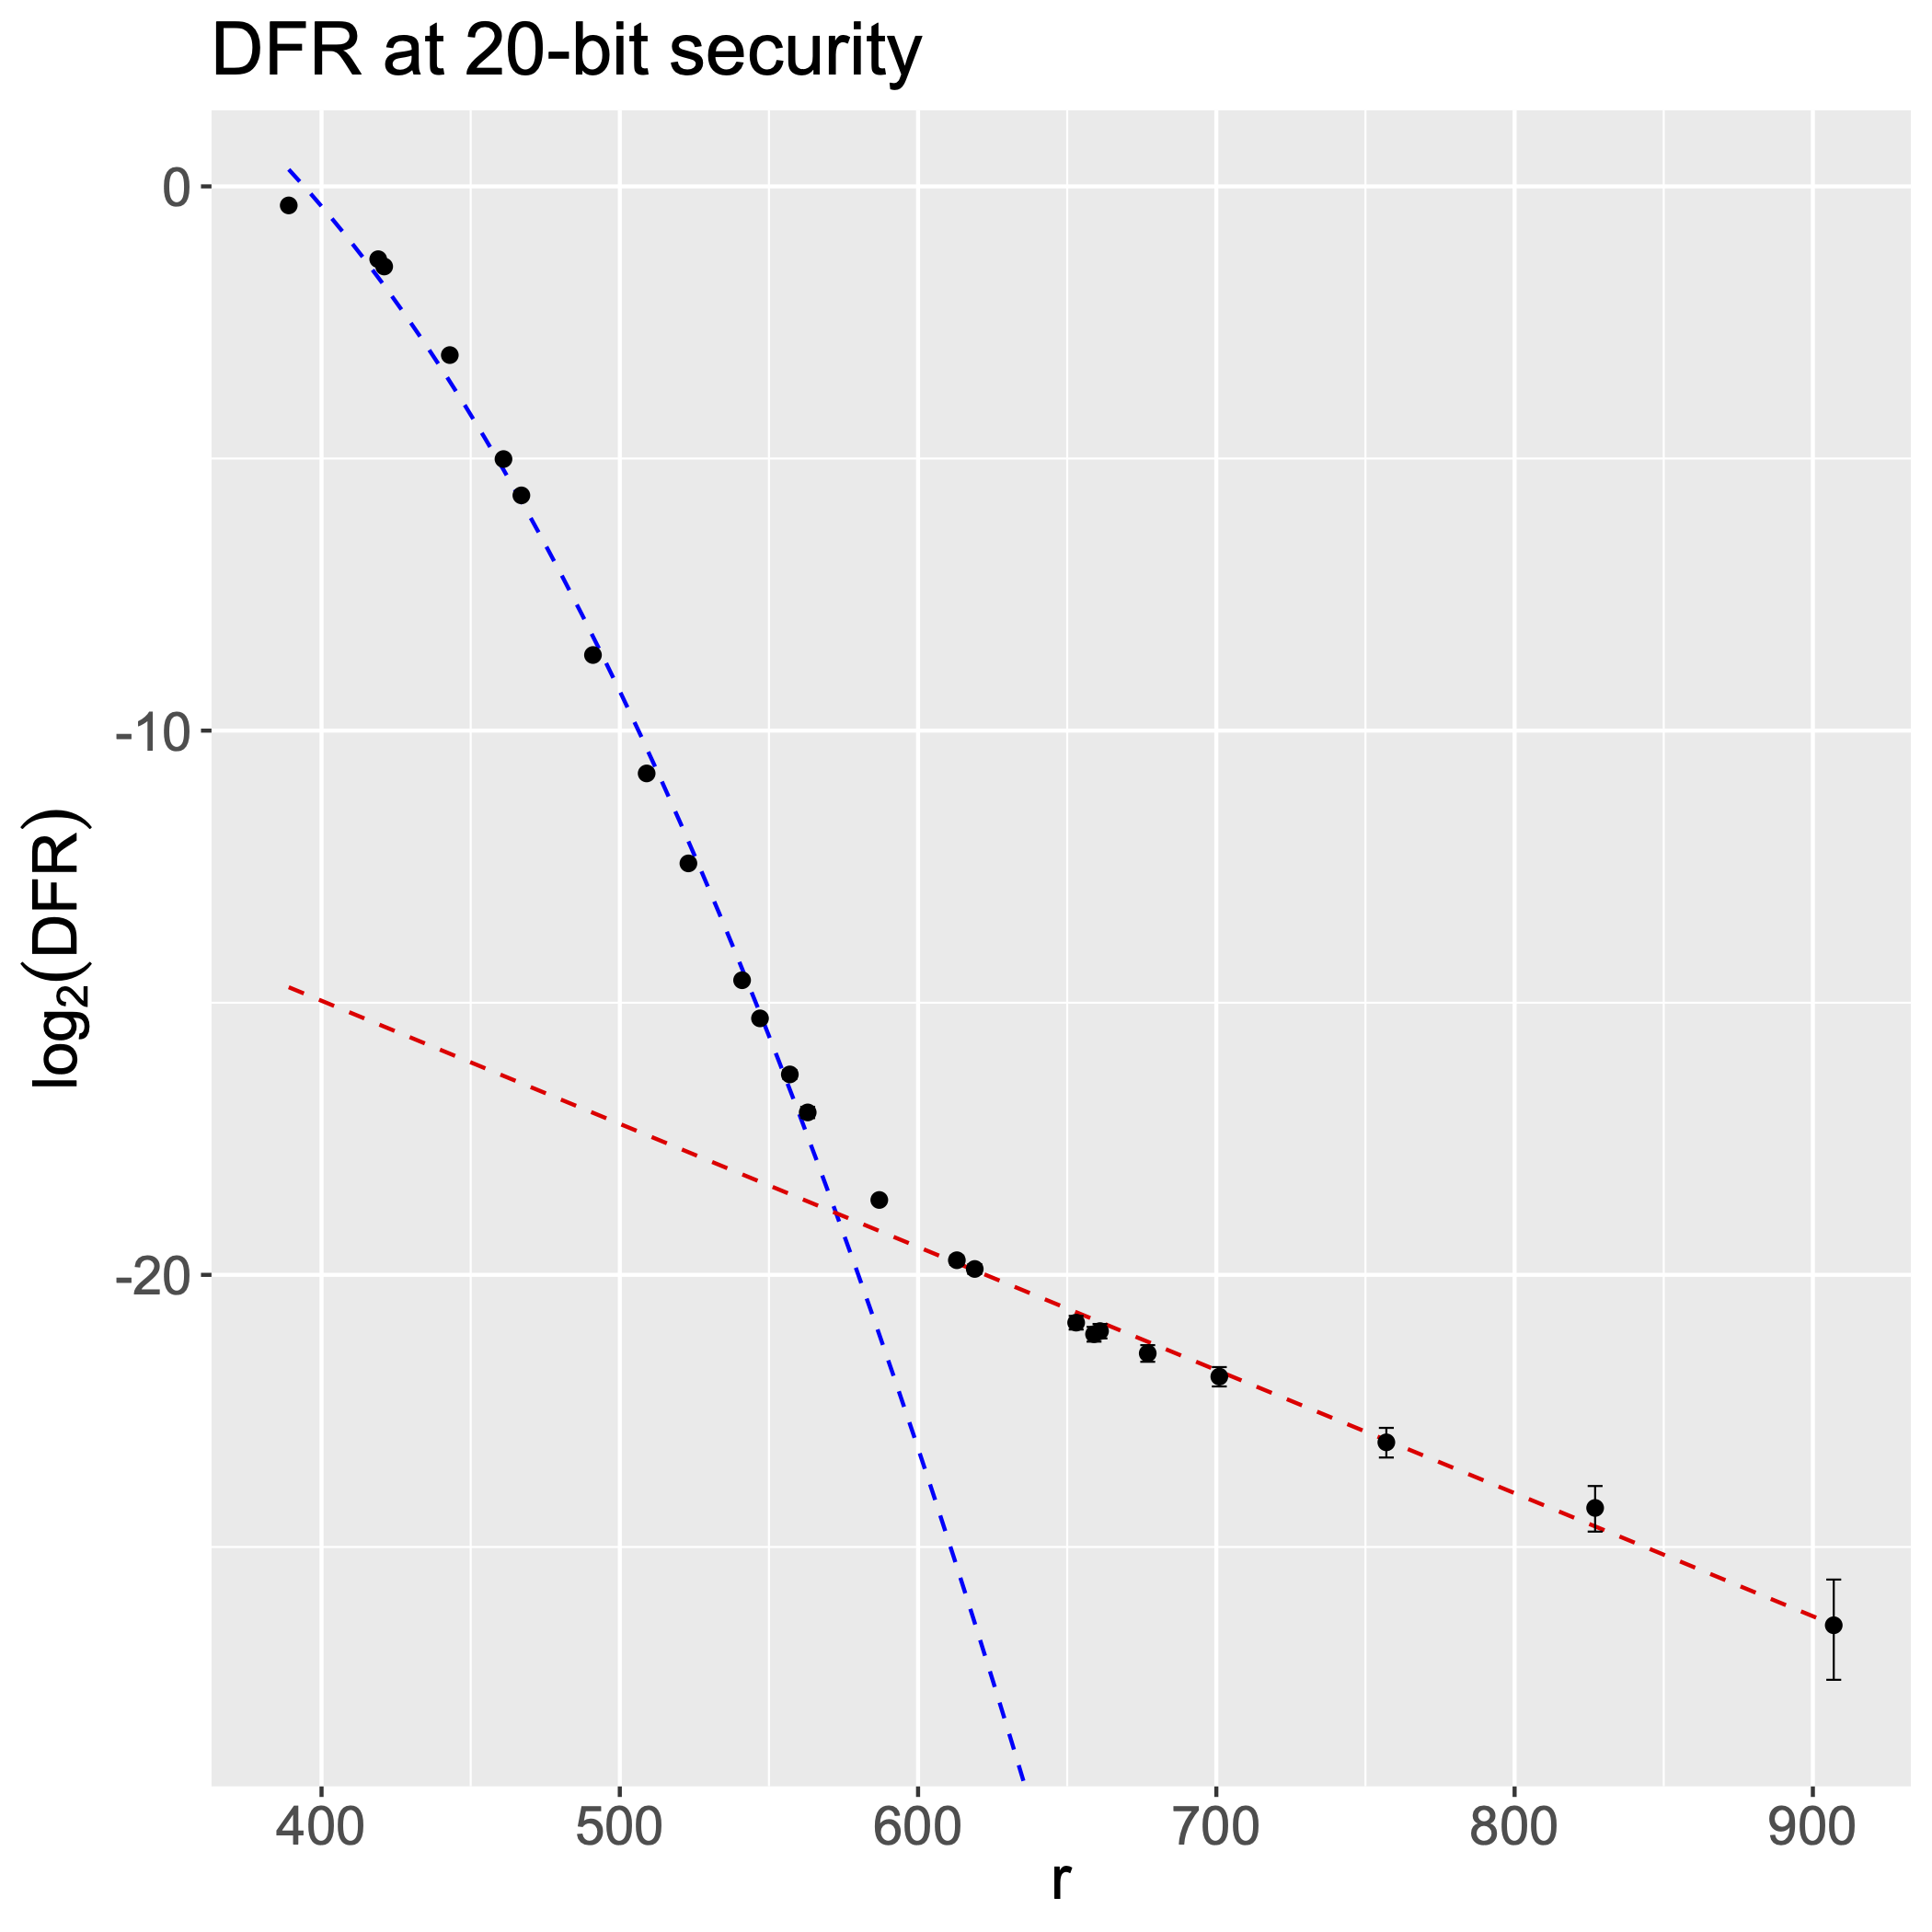
\includegraphics[width=0.49\textwidth]{2_bike/DFR-plot-random.png}
  \end{center}
  \caption{Semi-log plot of decoding failure rates for non-weak keys ($T = 3$, left) and for unfiltered random keys (right), with a 95\% confidence interval for each $r$. There is a quadratic best fit (blue) in the waterfall region and a linear best fit (red) in the error floor region ($r \geq 587$).}
  \label{fig:DFR}
\end{figure}


